% =====================================================================
%  B.Tech Project Final Evaluation Presentation
%
%  Compile with pdfLaTeX  (Overleaf: Menu -> Compiler -> pdfLaTeX)
%  Run twice so the Outline page picks up the section list.
%
%  Layout of this project:
%    preamble.tex        packages, beamer theme, colours, helper macros
%    titlepage.tex       title, authors, supervisor, institute
%    sections/*.tex      one file per section - edit these
%    figs/               all figures
% =====================================================================
\documentclass[aspectratio=169,10pt]{beamer}

% Packages, beamer theme and colour scheme for the deck.
% (\documentclass lives in main.tex)

\usetheme{Madrid}
\usepackage[T1]{fontenc}
\usepackage[utf8]{inputenc}
\usepackage{booktabs}
\usepackage{colortbl}
\usepackage{amsmath,amssymb}
\usepackage{graphicx}
\usepackage{tikz}
\usepackage{array}
% beamer already loads hyperref; just make the links visible
\hypersetup{colorlinks=true,urlcolor=astramBlue,linkcolor=astramInk,
            citecolor=astramInk}
\usetikzlibrary{arrows.meta,positioning,shapes.geometric,fit,backgrounds,calc}

% ---------- colour scheme ----------
\definecolor{astramInk}{RGB}{61,59,107}      % structure / headings
\definecolor{astramAmber}{RGB}{194,106,2}    % accent
\definecolor{astramRed}{RGB}{176,42,55}      % warnings
\definecolor{astramGreen}{RGB}{27,127,75}    % positives
\definecolor{astramBlue}{RGB}{43,89,138}
\definecolor{panelGrey}{RGB}{244,245,247}
\definecolor{boxBlue}{RGB}{228,237,246}
\definecolor{boxGreen}{RGB}{232,241,233}
\definecolor{boxAmber}{RGB}{253,240,226}
\definecolor{boxRed}{RGB}{253,242,242}
\definecolor{boxPurple}{RGB}{243,240,248}
\definecolor{leakYellow}{RGB}{255,249,219}

\setbeamercolor{structure}{fg=astramInk}
\setbeamercolor{alerted text}{fg=astramRed}
\setbeamercolor{block title}{bg=astramInk,fg=white}
\setbeamercolor{block title alerted}{bg=astramRed,fg=white}
\setbeamercolor{block title example}{bg=astramGreen,fg=white}
\setbeamercolor{block body example}{bg=boxGreen,fg=black}
\setbeamercolor{block body}{bg=panelGrey,fg=black}
\setbeamercolor{block body alerted}{bg=boxRed,fg=black}
\setbeamercolor{block body example}{bg=boxGreen}
\setbeamertemplate{blocks}[rounded][shadow=true]
\setbeamertemplate{navigation symbols}{}
\setbeamertemplate{itemize item}{\color{astramAmber}$\blacktriangleright$}
\setbeamertemplate{itemize subitem}{\color{astramAmber}\textbullet}
\setbeamerfont{block title}{size=\small}
\setbeamerfont{frametitle}{size=\large}

% tighter tables
\renewcommand{\arraystretch}{1.15}
\newcommand{\good}[1]{\textbf{\color{astramGreen}#1}}
\newcommand{\bad}[1]{\textbf{\color{astramRed}#1}}
\newcommand{\amb}[1]{\textbf{\color{astramAmber}#1}}
% \key{} = marker-pen highlight. Each word gets its own coloured box so the
% phrase can still break across lines (no soul/lua-ul dependency needed).
\definecolor{hlYellow}{RGB}{255,231,133}
\makeatletter
\newcommand{\key}[1]{\begingroup\setlength{\fboxsep}{1.6pt}%
  \@keyscan#1 \@nil\endgroup}
\def\@keyscan#1 #2\@nil{%
  \colorbox{hlYellow}{\strut#1}%
  \def\@keyrest{#2}%
  \ifx\@keyrest\@empty\else
    % coloured spacer sits flush against both words, so the stroke is
    % continuous; \allowbreak still lets the phrase wrap between words
    \nobreak\colorbox{hlYellow}{\strut\kern0.5pt}\allowbreak
    \@keyscan#2\@nil\fi}
\makeatother

% Title, authors, supervisor, institute.
\title[Congestion Severity Prediction]{Event-Driven Traffic Congestion Severity Prediction\\and Resource Recommendation System}
\author[Aman, Sahil, Vishwajit]{%
  Aman Kumar (2023IMT-010)\\
  Sahil Pal (2023IMT-069)\\
  Vishwajit Sarak Patil (2023IMT-071)\\[2mm]
  \small Supervisor: Dr.\ Saswata Roy}
\institute[ABV-IIITM Gwalior]{%
  Department of Information Technology\\
  ABV-Indian Institute of Information Technology and Management Gwalior}
\date[BTP Final Evaluation]{B.Tech Project: Final Evaluation Report}

% College logo shown on the title slide (vector PDF of the ABV-IIITM crest).
\titlegraphic{
\includegraphics[height=13mm]{figs/abv_iiitm_logo.pdf}}


\begin{document}

\input{sections/01-title-outline}
% Motivation
\section{Motivation}

\begin{frame}{Motivation: Why Event Severity?}
  \begin{columns}[T]
    \begin{column}{0.56\textwidth}
      \begin{itemize}
        \item \textbf{Non-recurring congestion} (accidents, breakdowns, public
              events) is the disruptive kind, and the hardest to plan for.
        \item When an event is first reported, the control room must decide
              \textbf{how much to send} (officers, barricades, diversions)
              \key{before anyone has seen the site}.
        \item That decision is currently made on \key{experience alone}.
        \item Under- or over-deploying both carry real cost: congestion on one
              side, wasted manpower on the other.
      \end{itemize}
    \end{column}
    \begin{column}{0.42\textwidth}
      \begin{block}{Operational impact}
        \begin{itemize}
          \item[\color{astramGreen}$\checkmark$] Faster first response
          \item[\color{astramGreen}$\checkmark$] Right-sized deployment
          \item[\color{astramGreen}$\checkmark$] Consistent decisions across shifts
        \end{itemize}
      \end{block}
      \begin{exampleblock}{Dataset at a glance}
        \small
        8{,}173 Bengaluru traffic events\\
        46 raw attributes $\rightarrow$ 30 engineered features\\
        4 severity classes
      \end{exampleblock}
    \end{column}
  \end{columns}
\end{frame}

% =====================================================================

% Problem background and positioning
\section{Problem Background}

\begin{frame}{The Gap in Existing Work}
  \begin{columns}[T]
    \begin{column}{0.55\textwidth}
      \textbf{What the literature does well:}
      \begin{itemize}
        \item Gradient-boosted trees perform consistently well on \key{tabular}
              incident-severity data.
        \item Deep learning for traffic congestion is mature, but focused on
              \emph{recurring}, sensor-driven flow.
        \item Stacked ensembles and imbalance-aware evaluation are each well
              established.
      \end{itemize}
      \vspace{2mm}
      \textbf{What is missing:}
      \begin{itemize}
        \item These three threads are rarely combined in one pipeline.
        \item Severity prediction almost never produces an \emph{operational
              recommendation}.
      \end{itemize}
    \end{column}
    \begin{column}{0.43\textwidth}
      \begin{block}{Positioning of this work}
        A stacked ensemble of tree-based \emph{and} neural classifiers applied to
        event-driven severity, evaluated with \key{front-loaded} attention to class
        imbalance, and coupled directly to a deterministic
        resource-recommendation engine.
      \end{block}
      \begin{alertblock}{Challenge}
        Severity is \key{not recorded anywhere} in the raw log. The target
        must be constructed, carefully.
      \end{alertblock}
    \end{column}
  \end{columns}
\end{frame}

% =====================================================================

% Target construction and the resulting class imbalance
\section{The Labelling Problem}

\begin{frame}[shrink]{Constructing a Target That Does Not Exist}
  \begin{center}\small
    No severity column exists in the raw log. The target is built by crossing two
    fields the control room records \emph{independently}, for its own purposes.
  \end{center}
  \vspace{-1mm}
  \centering
  \begin{tikzpicture}[font=\scriptsize,node distance=6mm,
    fld/.style={rounded corners=2pt,draw=astramBlue!60,fill=boxBlue,
                minimum height=7mm,text width=32mm,align=center},
    op/.style={circle,draw=astramInk!60,fill=white,inner sep=2pt},
    cls/.style={rounded corners=2pt,minimum height=5.4mm,text width=20mm,
                align=center,inner sep=1pt},
    ar/.style={-{Stealth[length=1.6mm]},astramAmber,thick}]
    \node[fld] (p) {\texttt{priority}\\ High / Low};
    \node[fld,below=5mm of p] (r) {\texttt{requires\_road\_closure}\\ Yes / No};
    \node[op] (cross) at ([xshift=13mm]$(p)!0.5!(r)$) {$\times$};
    \node[cls,draw=astramGreen!60,fill=boxGreen] (c0)
      at ([xshift=32mm,yshift=9mm]cross) {0 \ Low};
    \node[cls,draw=astramBlue!60,fill=boxBlue,below=1.4mm of c0]   (c1) {1 \ Medium};
    \node[cls,draw=astramAmber!70,fill=boxAmber,below=1.4mm of c1] (c2) {2 \ High};
    \node[cls,draw=astramRed!60,fill=boxRed,below=1.4mm of c2]     (c3) {3 \ Critical};
    \draw[ar] (p) -- (cross);
    \draw[ar] (r) -- (cross);
    \foreach \n in {c0,c1,c2,c3} \draw[ar] (cross) -- (\n.west);
  \end{tikzpicture}

  \vspace{2mm}
  \begin{columns}[T]
    \begin{column}{0.44\textwidth}
      \centering\small
      \setlength{\tabcolsep}{4pt}
      \begin{tabular}{clrr}
        \toprule
        Code & Label & Count & Share \\
        \midrule
        0 & Low      & 2{,}764 & 33.8\% \\
        1 & Medium   &   379   & \bad{4.6\%} \\
        2 & High     & 4{,}733 & 57.9\% \\
        3 & Critical &   297   & \bad{3.6\%} \\
        \bottomrule
      \end{tabular}

      \vspace{1mm}
      {\scriptsize Low and High are \key{91.7\%} of all events.}
    \end{column}
    \begin{column}{0.54\textwidth}
      \begin{alertblock}{Both source fields are then \emph{removed}}
        \small If left in the feature set, a model would simply re-learn this
        deterministic mapping instead of inferring severity from spatial,
        temporal and contextual signals, and would be \key{useless on a genuinely
        new, unassessed event}.
      \end{alertblock}
    \end{column}
  \end{columns}
\end{frame}

% Objectives
\section{Objectives}

\begin{frame}{Objectives}
  \vspace{2mm}
  \begin{enumerate}\setlength{\itemsep}{5mm}
    \item \textbf{Construct a four-class severity target} that the raw event log
          does not contain, \key{without leaking} the fields it was built from.
    \item \textbf{Engineer 30 spatial, temporal and contextual features},
          including an unsupervised K-Means clustering of event coordinates.
    \item \textbf{Train four classifiers and stack them} out-of-fold with a
          LightGBM meta-learner, comparing all five honestly.
    \item \textbf{Evaluate for class imbalance}, then convert the prediction
          into a resource recommendation and deploy it as a working service.
  \end{enumerate}
\end{frame}

% Dataset and missing-value audit
\section{Dataset and Features}

\begin{frame}{Dataset and Missing-Value Audit}
  \centering
  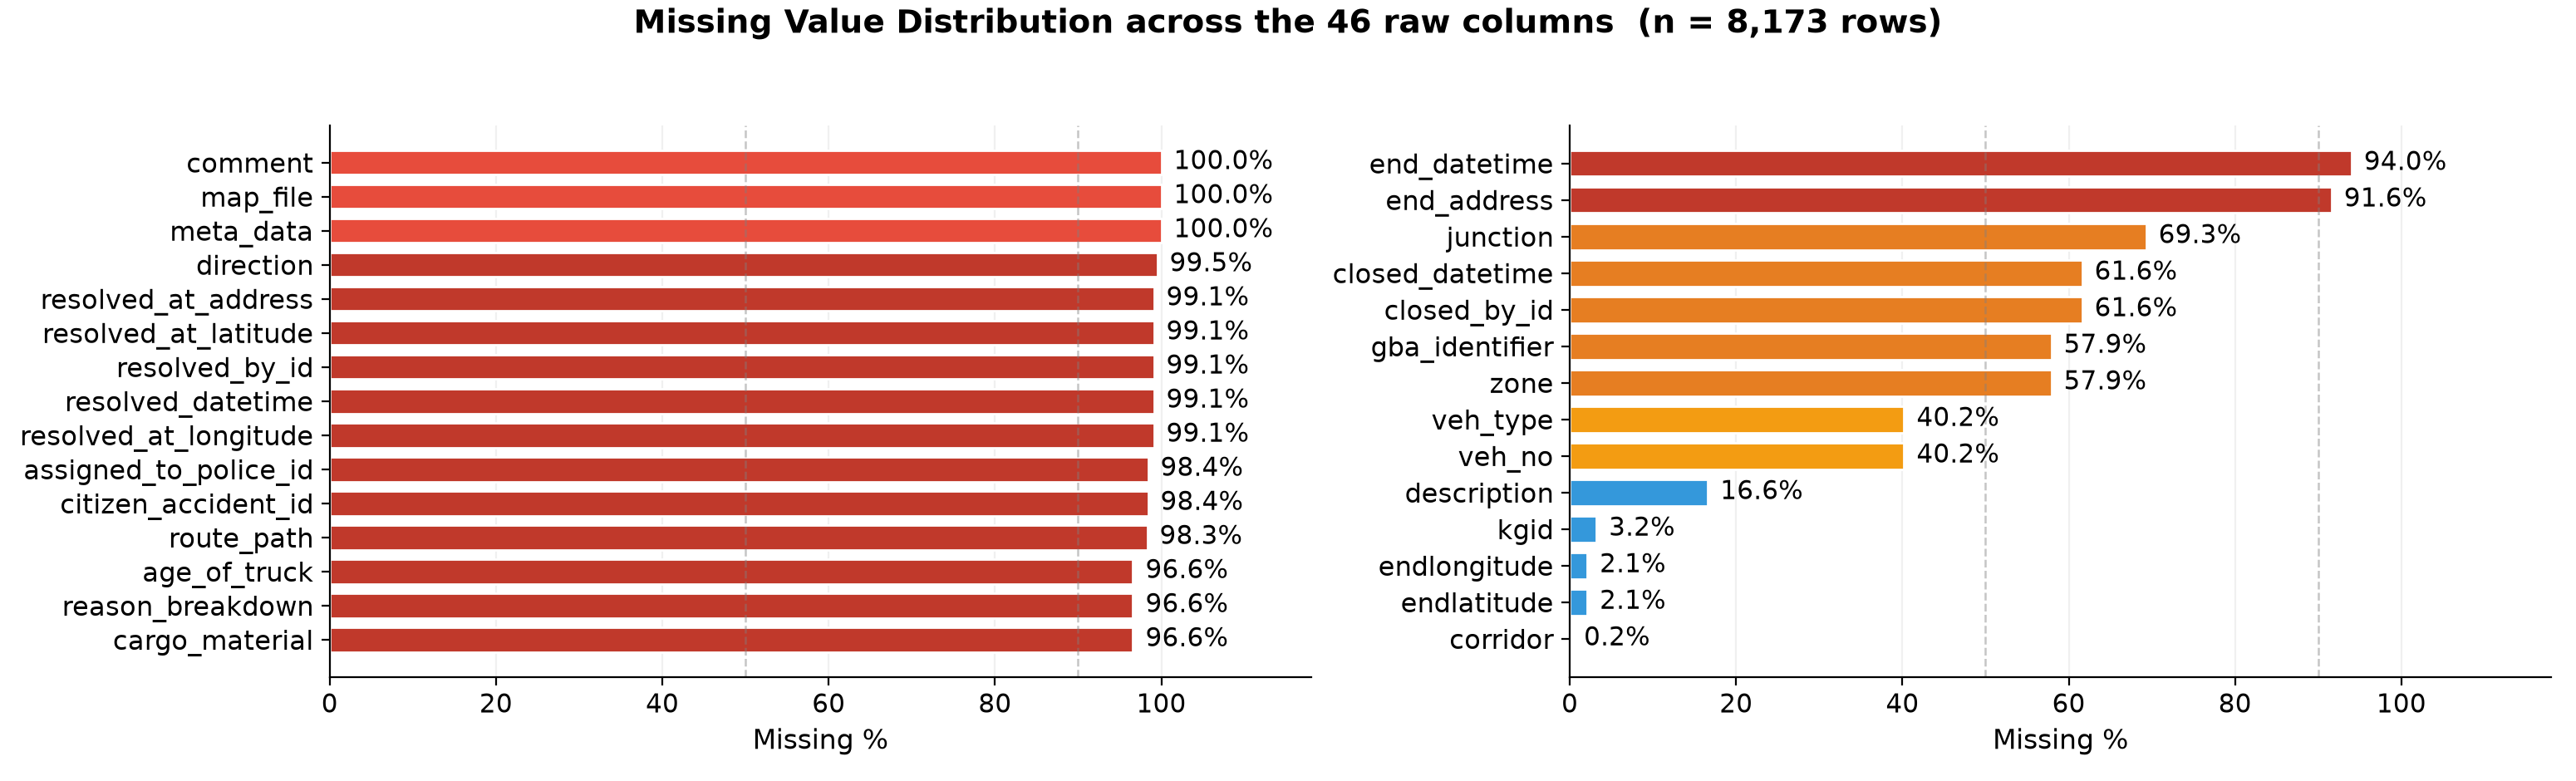
\includegraphics[width=0.95\textwidth]{figs/missing_values_wide.png}

  \vspace{2.5mm}
  \footnotesize
  \setlength{\tabcolsep}{5pt}
  \renewcommand{\arraystretch}{1.3}
  \begin{tabular}{>{\raggedright\arraybackslash}p{4.3cm}
                  >{\raggedright\arraybackslash}p{9.0cm}}
    \toprule
    Decision & Columns \\
    \midrule
    \bad{Dropped} \ (96--100\% missing) &
      \texttt{comment}, \texttt{map\_file}, \texttt{meta\_data}, resolution and
      truck fields \\
    \amb{Kept as ``unknown''} \ (40--70\%) &
      \texttt{junction}, \texttt{closed\_datetime}, \texttt{zone},
      \texttt{veh\_type} \\
    \good{Retained} \ (0\% missing) &
      coordinates, event cause, priority, closure flag \\
    \bad{Dropped} \ (identifiers) &
      \texttt{id}, \texttt{client\_id}, \texttt{created\_by\_id} \\
    \bottomrule
  \end{tabular}
\end{frame}

% Feature engineering and K-Means location clustering
\begin{frame}{Feature Engineering: 30 Features}
  \begin{columns}[T]
    \begin{column}{0.51\textwidth}
      \small
      \begin{tabular}{p{1.5cm}p{4.9cm}}
        \toprule
        Group & Features \\
        \midrule
        Spatial &
          latitude, longitude, corridor, police station, zone, junction,
          \textbf{location cluster} \\
        Temporal &
          hour, minute, day of week, month, day, weekend flag,
          morning- and evening-rush flags, time-of-day bucket \\
        Contextual &
          event type, event cause, vehicle type, duration, status,
          weather flag \\
        \bottomrule
      \end{tabular}

      \vspace{3mm}
      \begin{block}{Encoding and splitting}
        \small Nine categorical columns label-encoded, numerics standardised.
        Both transformers are \textbf{serialized}, so a new event is encoded exactly
        as in training. Split 6{,}538 / 1{,}635, \textbf{stratified}.
      \end{block}
    \end{column}
    \begin{column}{0.47\textwidth}
      \centering
      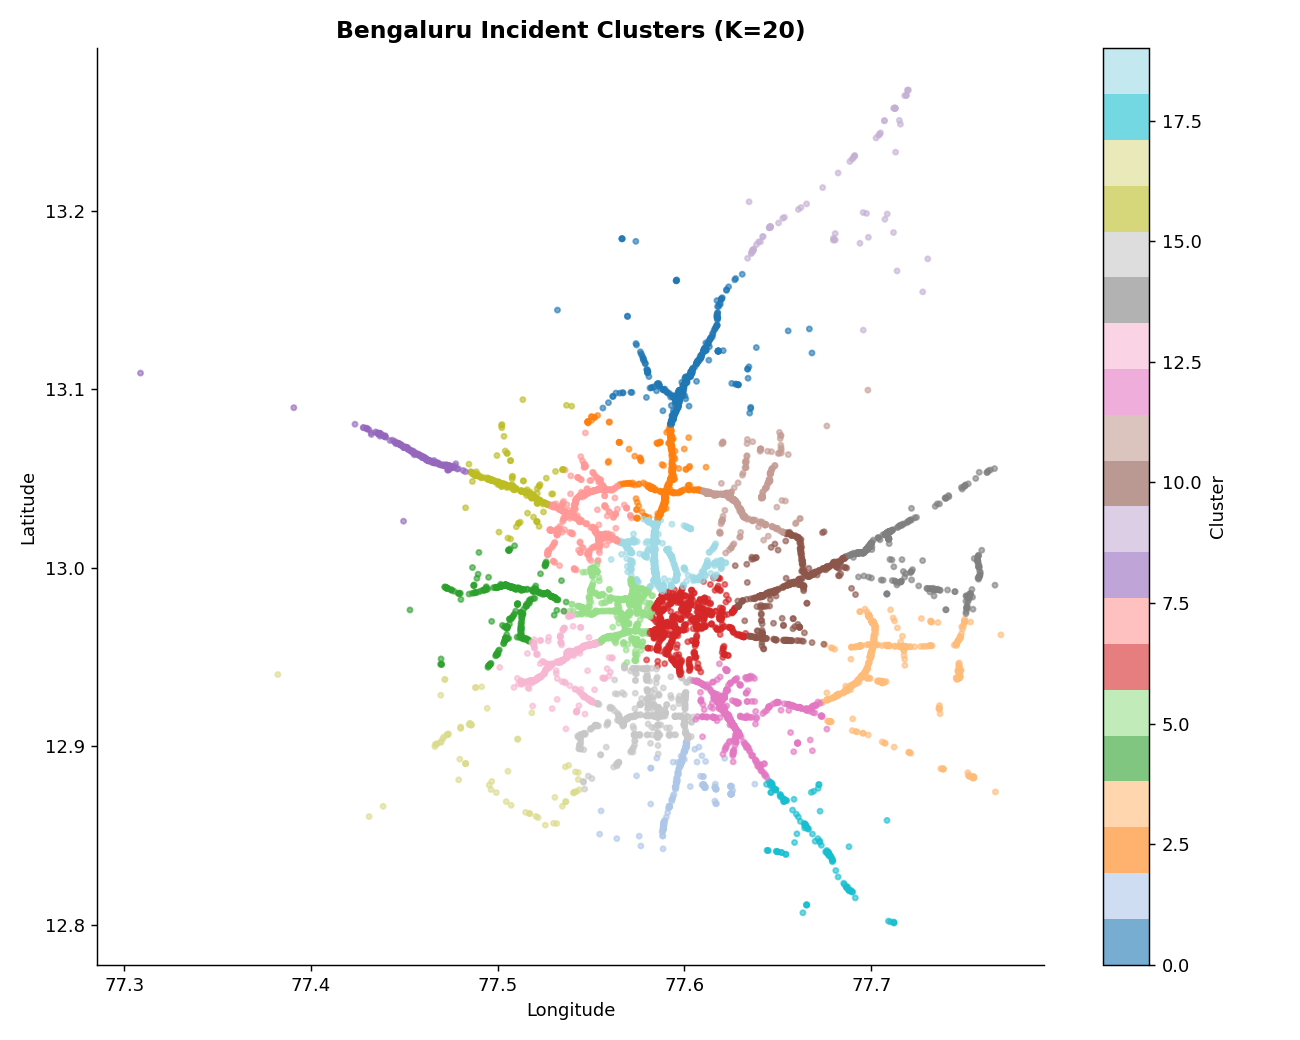
\includegraphics[width=\textwidth]{figs/geo_clusters.png}

      \vspace{1mm}
      {\scriptsize \textbf{K-Means, $K = 20$}: unsupervised grouping of the
      8{,}173 event coordinates; the cluster ID becomes feature 30.}
    \end{column}
  \end{columns}
\end{frame}

% Pipeline diagram and base learners
\section{Model Architecture}

\begin{frame}{Pipeline Overview: End-to-End Flow}
  \centering
  \begin{tikzpicture}[
      font=\small,
      >={Stealth[length=2.2mm]},
      stg/.style={rectangle,rounded corners=2.5pt,draw=astramBlue!70,fill=boxBlue,
                  minimum height=11mm,text width=20mm,align=center,inner sep=2pt,
                  line width=0.7pt},
      uns/.style={stg,draw=astramInk!60,fill=boxPurple},
      mdl/.style={stg,draw=astramGreen!70,fill=boxGreen,text width=27mm},
      nn/.style={mdl,draw=astramAmber!80,fill=boxAmber},
      bar/.style={rectangle,rounded corners=2.5pt,draw=black!35,fill=panelGrey,
                  minimum height=10mm,text width=112mm,align=center,inner sep=2pt},
      meta/.style={mdl,text width=44mm,minimum height=12mm},
      fin/.style={stg,draw=astramRed!70,fill=boxRed,text width=48mm,
                  minimum height=12mm,line width=1pt},
      num/.style={font=\bfseries},
      ar/.style={->,astramAmber,line width=1pt}]

    % ---------- row 1 : data preparation ----------
    \node[stg] (raw) at (0,0)      {\textbf{1.} Raw log\\[-0.3mm]{\scriptsize 8{,}173 $\times$ 46}};
    \node[stg] (cln) at (2.55,0)   {\textbf{2.} Cleaning\\[-0.3mm]{\scriptsize impute / drop}};
    \node[stg] (fe)  at (5.10,0)   {\textbf{3.} Features\\[-0.3mm]{\scriptsize 30 engineered}};
    \node[uns] (km)  at (7.65,0)   {\textbf{4.} K-Means\\[-0.3mm]{\scriptsize $K = 20$}};
    \node[stg] (enc) at (10.20,0)  {\textbf{5.} Encode\\[-0.3mm]{\scriptsize + scale}};
    \node[stg] (spl) at (12.75,0)  {\textbf{6.} Split\\[-0.3mm]{\scriptsize 80 / 20}};
    \foreach \a/\b in {raw/cln,cln/fe,fe/km,km/enc,enc/spl} \draw[ar] (\a) -- (\b);

    % ---------- row 2 : four base learners ----------
    \node[mdl] (lgb) at (1.7,-2.05)  {\textbf{7.} LightGBM\\[-0.3mm]{\scriptsize\itshape class-weighted}};
    \node[mdl] (xgb) at (5.15,-2.05) {\textbf{7.} XGBoost\\[-0.3mm]{\scriptsize\itshape class-weighted}};
    \node[nn]  (mlp) at (8.60,-2.05) {\textbf{7.} MLP\\[-0.3mm]{\scriptsize 256-128-64-32}};
    \node[nn]  (tab) at (12.05,-2.05){\textbf{7.} TabNet\\[-0.3mm]{\scriptsize attentive}};
    \coordinate (busA) at (12.75,-1.15);
    \draw[astramAmber,line width=1pt] (spl.south) -- (busA);
    \draw[astramAmber,line width=1pt] (1.7,-1.15) -- (12.75,-1.15);
    \foreach \n in {lgb,xgb,mlp,tab} \draw[ar] (\n |- busA) -- (\n.north);

    % ---------- row 3 : stacked meta-features ----------
    \node[bar] (m16) at (6.4,-3.95)
      {\textbf{8.} 16 meta-features $=$ 4 models $\times$ 4 class probabilities,
       generated \textbf{out-of-fold}};
    \coordinate (busB) at (6.4,-3.05);
    \draw[astramAmber,line width=1pt] (1.7,-3.05) -- (12.05,-3.05);
    \foreach \n in {lgb,xgb,mlp,tab} \draw[astramAmber,line width=1pt] (\n.south) -- (\n |- busB);
    \draw[ar] (busB) -- (m16.north);

    % ---------- row 4 : meta-learner and final output ----------
    \node[meta] (meta) at (2.9,-5.85)
      {\textbf{9.} Meta-learner\\[-0.3mm]{\scriptsize LightGBM}};
    \node[fin]  (out)  at (9.9,-5.85)
      {\textbf{10.} Severity 0--3 $+$ confidence\\[-0.3mm]{\scriptsize $\rightarrow$ rule engine}};
    \draw[ar] (m16.south) -- ++(0,-0.45) -| (meta.north);
    \draw[ar] (meta) -- (out);
  \end{tikzpicture}

  \vspace{1mm}
  {\scriptsize Steps 1--9 are learned; the rule engine after step 10 is deterministic.}

\end{frame}

\begin{frame}{Base Learners: Two Very Different Styles}
  \begin{columns}[T]
    \begin{column}{0.5\textwidth}
      \begin{exampleblock}{Gradient-boosted trees: LightGBM and XGBoost}
        \small Hundreds of shallow decision trees built \emph{in sequence}, each
        one specialising in the mistakes the previous trees made.
      \end{exampleblock}

      \vspace{1mm}
      \centering
      \begin{tikzpicture}[font=\scriptsize,>={Stealth[length=1.8mm]},
        t/.style={draw=astramGreen!70,fill=white,rounded corners=2pt,
                  minimum height=11mm,text width=17mm,align=center,inner sep=1.5pt},
        ar/.style={->,astramGreen,line width=0.9pt}]
        \node[t] (t1) at (0,0)    {\textbf{Tree 1}\\[-0.3mm]{\scriptsize first guess}};
        \node[t] (t2) at (2.15,0) {\textbf{Tree 2}\\[-0.3mm]{\scriptsize fixes T1}};
        \node[t] (t3) at (4.30,0) {\textbf{Tree 3}\\[-0.3mm]{\scriptsize fixes T2}};
        \node[font=\scriptsize] (td) at (5.75,0) {$\cdots \times 1000$};
        \draw[ar] (t1)--(t2); \draw[ar] (t2)--(t3); \draw[ar] (t3)--(td);
      \end{tikzpicture}

      \vspace{2mm}
      \begin{block}{Configuration}
        \small 1000 estimators, learning rate 0.03. LightGBM grows leaf-wise
        (63 leaves), XGBoost depth-wise (depth 6). \textbf{Both use
        class-balanced sample weighting.}
      \end{block}
    \end{column}
    \begin{column}{0.47\textwidth}
      \begin{block}{Neural approaches: MLP and TabNet}
        \small Layers of neurons pass weighted signals forward; the weights are
        adjusted over many passes to reduce error.
      \end{block}

      \vspace{1mm}
      \centering
      \begin{tikzpicture}[font=\scriptsize,>={Stealth[length=1.6mm]},
        n/.style={circle,draw=astramAmber!80,fill=boxAmber,minimum size=3.2mm,
                  inner sep=0pt},
        lbl/.style={font=\scriptsize,text=astramInk}]
        \foreach \c/\k in {0/4,1/3,2/3,3/2}{
          \foreach \r in {1,...,\k}{
            \node[n] at ({1.35*\c},{-0.42*\r+0.21*\k}) {};
          }
        }
        \foreach \c/\w in {0/256,1/128,2/64,3/32}
          \node[lbl] at ({1.35*\c},-1.15) {\w};
        \foreach \c in {0,1,2}
          \draw[->,astramAmber,line width=0.8pt]
            ({1.35*\c+0.35},0) -- ({1.35*\c+1.0},0);
      \end{tikzpicture}

      \vspace{1mm}
      {\scriptsize MLP hidden layers. TabNet instead uses \textbf{attention}
      over 5 decision steps.}

      \vspace{1mm}
      \begin{alertblock}{Class weighting: the deciding choice}
        \small\vspace{-2mm}
        \[ w_c = \frac{n}{C\, n_c} \qquad
           \frac{w_{\text{Critical}}}{w_{\text{High}}} \approx 16 \]
        \small Applied to the two tree models, \textbf{not} the neural ones.
      \end{alertblock}
    \end{column}
  \end{columns}
\end{frame}

% Out-of-fold stacked generalization
\section{Stacked Generalization}

\begin{frame}[shrink]{Stacking Without Leakage}
  \begin{alertblock}{The problem}
    A model that has \textbf{already seen} an event predicts it far too
    confidently. Training the meta-learner on those inflated probabilities
    teaches it to trust an accuracy that \textbf{will not exist} on real new
    events.
  \end{alertblock}

  \begin{columns}[T]
    \begin{column}{0.55\textwidth}
      \centering
      \begin{tikzpicture}[font=\scriptsize,
        tr/.style={draw=astramBlue!50,fill=boxBlue,minimum width=11.5mm,
                   minimum height=5mm,inner sep=1pt},
        pr/.style={tr,draw=astramAmber!70,fill=boxAmber}]
        \foreach \r in {1,...,5}{
          \node[anchor=east] at (-0.2,{-0.62*\r}) {Fold \r};
          \foreach \c in {1,...,5}{
            \pgfmathparse{int(\r==\c)}
            \ifnum\pgfmathresult=1
              \node[pr] at ({1.30*\c},{-0.62*\r}) {predict};
            \else
              \node[tr] at ({1.30*\c},{-0.62*\r}) {train};
            \fi
          }
        }
      \end{tikzpicture}

      \vspace{2mm}
      {\scriptsize In each fold, fresh copies of \textbf{all four} base models
      train on the blue slices and predict the orange one.}
    \end{column}
    \begin{column}{0.43\textwidth}
      \begin{exampleblock}{Out-of-fold matrix}
        \small\vspace{-2mm}
        \[ z_i = \big[\, p^{(1)}_i \,\|\, p^{(2)}_i \,\|\, p^{(3)}_i
                        \,\|\, p^{(4)}_i \,\big] \in \mathbb{R}^{16} \]
        \small $p^{(m)}_i$ is model $m$'s class-probability vector for event $i$,
        from the fold that \textbf{excluded} $i$. Stacked: $6{,}538 \times 16$.
      \end{exampleblock}
      \begin{block}{Meta-learner}
        \small A LightGBM trained on those 16 columns, learning how much to trust
        each base model rather than averaging them naively.
      \end{block}
    \end{column}
  \end{columns}
\end{frame}

% =====================================================================

% Precision, recall and why accuracy misleads on imbalanced data
\section{Evaluation Methodology}

\begin{frame}{Why Accuracy Is the Wrong Headline Metric}
  \centering
  \begin{tikzpicture}[font=\small,
    cell/.style={rounded corners=2pt,minimum width=32mm,minimum height=15mm,
                 align=center,inner sep=2pt},
    hdr/.style={font=\scriptsize\bfseries,align=center}]

    % column / row headings
    \node[hdr] at (0,1.05)  {Predicted\\Critical};
    \node[hdr] at (3.6,1.05) {Predicted\\Not Critical};
    \node[hdr,anchor=east] at (-1.95,0)    {Actually\\Critical (59)};
    \node[hdr,anchor=east] at (-1.95,-1.8) {Actually\\Not (1{,}576)};

    % the four cells
    \node[cell,draw=astramGreen!60,fill=boxGreen] at (0,0)
      {{\Large\bfseries\color{astramGreen}2}\\[-0.5mm]{\scriptsize caught (TP)}};
    \node[cell,draw=astramRed!70,fill=boxRed,line width=1pt] at (3.6,0)
      {{\Large\bfseries\color{astramRed}57}\\[-0.5mm]{\scriptsize \textbf{missed} (FN)}};
    \node[cell,draw=black!25,fill=panelGrey] at (0,-1.8)
      {{\Large\bfseries 0}\\[-0.5mm]{\scriptsize false alarms (FP)}};
    \node[cell,draw=black!25,fill=panelGrey] at (3.6,-1.8)
      {{\Large\bfseries 1{,}576}\\[-0.5mm]{\scriptsize correctly calm (TN)}};

    % metrics read off the matrix
    \node[anchor=west,align=left,text width=52mm] at (6.0,0.15)
      {\textbf{Precision} $=\dfrac{TP}{TP+FP}=\dfrac{2}{2}=$
       \textbf{\color{astramInk}1.00}\\[1mm]
       {\scriptsize Of what it \emph{called} Critical, how much was?}};
    \node[anchor=west,align=left,text width=52mm] at (6.0,-1.75)
      {\textbf{Recall} $=\dfrac{TP}{TP+FN}=\dfrac{2}{59}=$
       \textbf{\color{astramRed}0.03}\\[1mm]
       {\scriptsize Of what \emph{truly was} Critical, how much did it catch?}};
  \end{tikzpicture}

  \vspace{3mm}
  \begin{columns}[T]
    \begin{column}{0.5\textwidth}
      \begin{alertblock}{The trap: MLP on the Critical class}
        \small \textbf{92.4\% accurate, 3\% Critical recall.} 91.7\% of events
        are Low or High, so a model can lean on those two and still be blind to
        the class the system exists to catch.
      \end{alertblock}
    \end{column}
    \begin{column}{0.48\textwidth}
      \begin{exampleblock}{Therefore: macro-F1, not accuracy}
        \vspace{-4mm}
        \[ F1_c = \frac{2 P_c R_c}{P_c + R_c}, \qquad
           \text{macro-F1} = \frac{1}{C}\textstyle\sum_{c=1}^{C} F1_c \]
        \small Every class counts equally, so ignoring Critical is punished.
      \end{exampleblock}
    \end{column}
  \end{columns}
\end{frame}

% Results, per-class, ensemble, importances
\section{Results}

\begin{frame}{Overall Results on 1{,}635 Held-Out Events}
  \begin{columns}[T]
    \begin{column}{0.54\textwidth}
      \centering\small
      \setlength{\tabcolsep}{4pt}
      \begin{tabular}{lccc}
        \toprule
        Model & Acc. & Macro-F1 & Wtd-F1 \\
        \midrule
        LightGBM         & 0.9223 & \good{0.6949} & 0.9148 \\
        XGBoost          & 0.9168 & 0.6906 & 0.9114 \\
        MLP-NN           & 0.9242 & \bad{0.5843} & 0.8992 \\
        TabNet           & \amb{0.9254} & 0.6027 & 0.9020 \\
        Stacked Ensemble & 0.8948 & 0.6639 & 0.8968 \\
        \bottomrule
      \end{tabular}

      \vspace{3mm}
      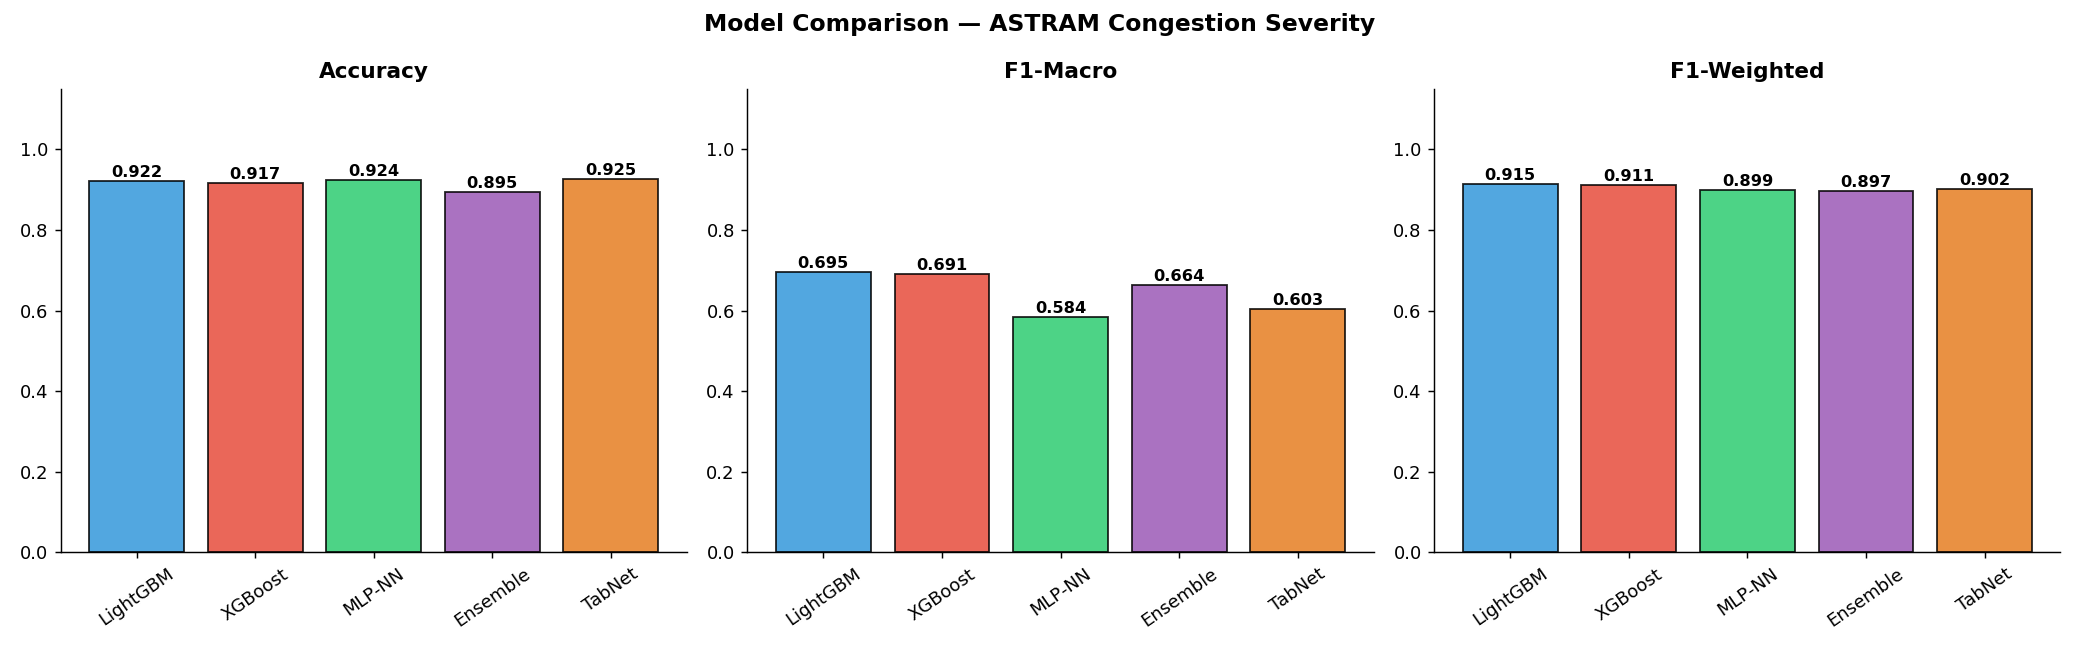
\includegraphics[width=0.95\textwidth]{figs/model_comparison.png}
    \end{column}
    \begin{column}{0.44\textwidth}
      \begin{block}{A narrow accuracy band}
        \small Every model sits between 89\% and 93\% accuracy, a spread that
        looks unremarkable. Macro-F1 ranges from 0.5843 to 0.6949, a gap far too
        wide to be explained by those near-identical accuracies.
      \end{block}
      \begin{alertblock}{The reversal}
        \small TabNet posts the \textbf{highest accuracy}. LightGBM has the
        \textbf{best macro-F1}. Ranking these models by accuracy would point a
        deployment decision at the wrong model.
      \end{alertblock}
    \end{column}
  \end{columns}
\end{frame}

\begin{frame}[shrink=5]{Per-Class Results: Where the Spread Comes From}
  \begin{columns}[T]
    \begin{column}{0.48\textwidth}
      \centering
      \textbf{Critical class} (support $=$ 59)\\[1mm]
      \begin{tabular}{lccc}
        \toprule
        Model & Prec. & Recall & F1 \\
        \midrule
        LightGBM         & 0.54 & 0.32 & \good{0.40} \\
        XGBoost          & 0.46 & \good{0.36} & \good{0.40} \\
        MLP-NN           & 1.00 & \bad{0.03} & \bad{0.07} \\
        TabNet           & 0.75 & \bad{0.10} & 0.18 \\
        Stacked Ensemble & 0.28 & 0.34 & 0.31 \\
        \bottomrule
      \end{tabular}

      \vspace{3mm}
      \textbf{Medium class} (support $=$ 76)\\[1mm]
      \begin{tabular}{lccc}
        \toprule
        Model & Prec. & Recall & F1 \\
        \midrule
        LightGBM         & 0.58 & 0.39 & \good{0.47} \\
        XGBoost          & 0.56 & 0.39 & 0.46 \\
        MLP-NN           & 0.75 & 0.24 & 0.36 \\
        TabNet           & 0.83 & 0.20 & \bad{0.32} \\
        Stacked Ensemble & 0.49 & \good{0.46} & \good{0.47} \\
        \bottomrule
      \end{tabular}
    \end{column}
    \begin{column}{0.5\textwidth}
      \begin{exampleblock}{Key finding}
        \small The only two models with \emph{usable} Critical recall,
        LightGBM (0.32) and XGBoost (0.36), are \textbf{exactly the two
        trained with class-balanced weighting}.
      \end{exampleblock}
      \begin{block}{Majority classes are easy}
        \small Every model handles Low (F1 0.93--0.94) and High (F1 0.95--0.97)
        comfortably. The entire macro-F1 spread comes from the two rare classes
        exactly what accuracy hides.
      \end{block}
      \begin{alertblock}{Honest note on stacking}
        \small The ensemble posts the \emph{lowest} accuracy of the five
        (0.8948). Its in-fold models were lighter, and each fold holds under
        100 rare-class examples. It still reaches the second-best Critical
        recall.
      \end{alertblock}
    \end{column}
  \end{columns}
\end{frame}



\begin{frame}[shrink]{Feature Importances}
  \begin{columns}[T]
    \begin{column}{0.52\textwidth}
      \centering
      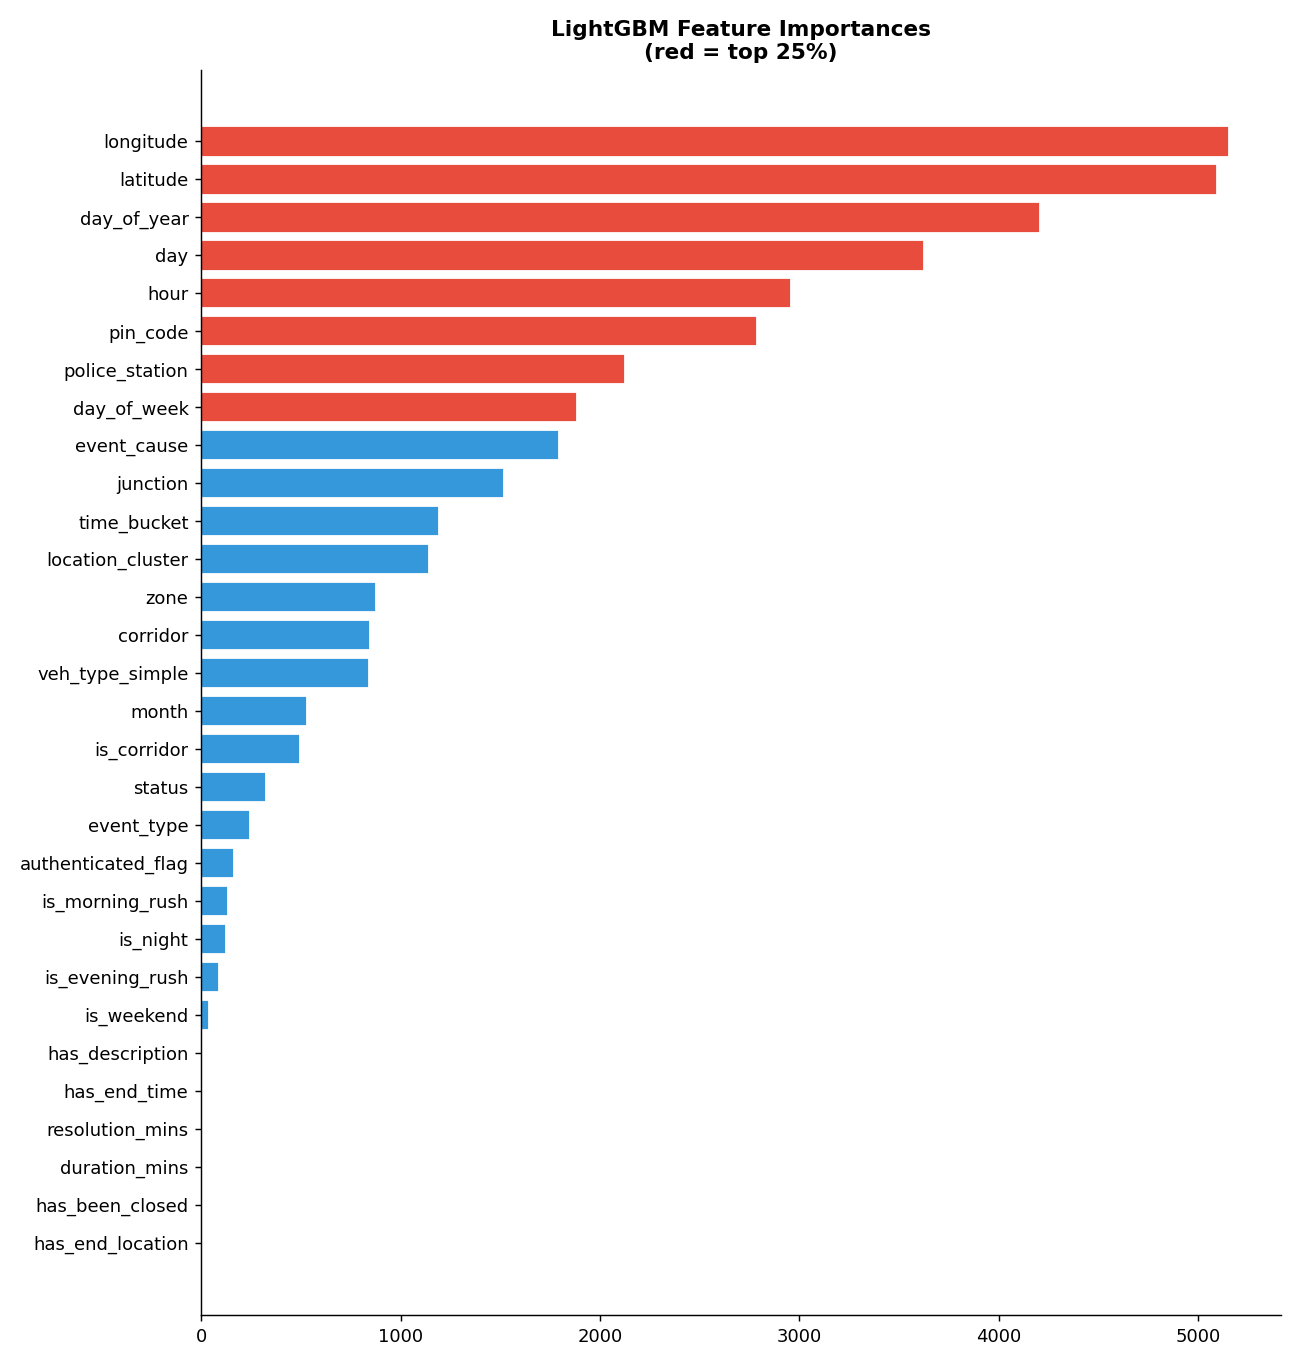
\includegraphics[width=\textwidth]{figs/lgbm_feature_importance.png}\\
      {\scriptsize LightGBM split-based importance; red bars mark the top
      quartile.}
    \end{column}
    \begin{column}{0.46\textwidth}
      \begin{block}{What ranks highest}
        \small
        \begin{itemize}
          \item \textbf{Raw coordinates dominate}: \texttt{longitude} and
                \texttt{latitude} are the two most-used split features.
          \item \textbf{Fine-grained time next}: \texttt{day\_of\_year},
                \texttt{day}, \texttt{hour}.
          \item \textbf{Then jurisdiction and cause}: \texttt{pin\_code},
                \texttt{police\_station}, \texttt{day\_of\_week},
                \texttt{event\_cause}.
        \end{itemize}
      \end{block}
      \begin{alertblock}{Caveat}
        \small Split-count importance favours \textbf{high-cardinality}
        features. That is why the engineered binary flags
        (\texttt{is\_corridor}, \texttt{is\_weekend}, rush-hour) sit at the
        bottom: it counts how \emph{often} a feature is split on, not the size or
        direction of its effect.
      \end{alertblock}
    \end{column}
  \end{columns}
\end{frame}

% =====================================================================

% Rule engine and worked example
\section{Recommendation Engine}

\begin{frame}{From Severity to a Deployment Plan}
  \begin{block}{Separation of concerns}
    \small The models answer \emph{how severe}; the rule engine answers
    \emph{what to do}. Deterministic and separate, so it stays auditable and
    tunable \textbf{without retraining}.
  \end{block}

  \vspace{1mm}
  \centering\small
  \setlength{\tabcolsep}{5pt}
  \begin{tabular}{lccll}
    \toprule
    Severity & Officers & Delay & Barricading & Diversion \\
    \midrule
    Low            & 2--4         & 15 min & Cones and indicators
                   & None \\
    Medium         & 4--8         & 30 min & Partial, 1 lane $+$ marshal
                   & Advisory alternate route \\
    High           & 8--14        & 60 min & Full, both sides $+$ 2 marshals
                   & Mandatory $+$ signage \\
    \bad{Critical} & \bad{15--25} & 90 min & Corridor lockdown $+$ chain
                   & Police-escorted $+$ advisory \\
    \bottomrule
  \end{tabular}

  \vspace{3mm}
  \begin{columns}[T]
    \begin{column}{0.44\textwidth}
      \begin{exampleblock}{Contextual multipliers}
        \begin{minipage}[t][13mm][t]{\linewidth}
          \small\vspace{-2mm}
          \[ n = \big\lfloor \lfloor n_{\text{base}}\, 1.4^{\,c} \rfloor\, 1.25^{\,p} \big\rfloor \]
          \small $c, p \in \{0,1\}$: corridor, peak (7--10, 17--21).
        \end{minipage}
      \end{exampleblock}
    \end{column}
    \begin{column}{0.54\textwidth}
      \begin{block}{Cause-specific actions}
        \begin{minipage}[t][13mm][t]{\linewidth}
          \small \texttt{accident} $\geq$ High: ambulance lane open, trauma
          centre on standby. \texttt{public\_event} $\geq$ High: crowd-control
          perimeter. Pre-announced: deploy 2\,h early.
        \end{minipage}
      \end{block}
    \end{column}
  \end{columns}
\end{frame}

\begin{frame}{Worked Example: One Event End to End}
  \centering
  \begin{tikzpicture}[
      font=\small, >={Stealth[length=2.6mm]},
      hd/.style={rectangle,text=white,text width=30mm,minimum height=6.5mm,
                 align=center,inner sep=1.5pt,font=\small\bfseries},
      bd/.style={rectangle,text width=30mm,minimum height=24mm,align=left,
                 inner sep=3pt,anchor=north,font=\scriptsize},
      cd/.style={rounded corners=2.5pt,line width=1pt,inner sep=0pt},
      ar/.style={->,astramAmber,line width=1.3pt}]

    \node[hd,fill=astramBlue!75] (h0) at (0,0) {1.~Event reported};
    \node[bd,fill=boxBlue] (b0) at (h0.south) {cause: accident\\ time: 18:30 Tue\\ corridor: ORR\\ duration: 90 min\\[1mm]
       \emph{as first logged}};
    \node[cd,draw=astramBlue!70,fit=(h0)(b0)] (c0) {};
    \node[hd,fill=astramInk!75] (h4) at (4,0) {2.~Feature vector};
    \node[bd,fill=boxPurple] (b4) at (h4.south) {cause $\rightarrow$ encoded\\ 18:30 $\rightarrow$ evening peak\\
       lat/long $\rightarrow$ cluster 7\\[1mm] \emph{30 features assembled}};
    \node[cd,draw=astramInk!60,fit=(h4)(b4)] (c4) {};
    \node[hd,fill=astramGreen!75] (h8) at (8,0) {3.~Base models};
    \node[bd,fill=boxGreen] (b8) at (h8.south) {LightGBM \hfill 0.71\\ XGBoost \hfill 0.68\\ MLP \hfill 0.62\\
       TabNet \hfill 0.65\\[1mm] \emph{stacked by meta-learner}};
    \node[cd,draw=astramGreen!70,fit=(h8)(b8)] (c8) {};
    \node[hd,fill=astramRed!75] (h12) at (12,0) {4.~Verdict};
    \node[bd,fill=boxRed] (b12) at (h12.south) {\centering\vspace{0.5mm}
       {\Large\bfseries\color{astramRed} HIGH}\\[1.5mm]
       severity 2 of 3\\ confidence 0.71\par};
    \node[cd,draw=astramRed!70,fit=(h12)(b12)] (c12) {};

    \draw[ar] (c0) -- (c4);
    \draw[ar] (c4) -- (c8);
    \draw[ar] (c8) -- (c12);
  \end{tikzpicture}

  \vspace{3mm}
  \begin{columns}[T]
    \begin{column}{0.46\textwidth}
      \begin{exampleblock}{5. Rule engine (deterministic)}
        \begin{minipage}[t][14mm][t]{\linewidth}
          \small Base for High: \texttt{8--14}\\
          $\lfloor 8(1.4)\rfloor = 11,\ \lfloor 11(1.25)\rfloor = 13$\\
          $\lfloor 14(1.4)\rfloor = 19,\ \lfloor 19(1.25)\rfloor = 23$\\[1mm]
          $\Rightarrow$ {\large\amb{13--23 officers}}
        \end{minipage}
      \end{exampleblock}
    \end{column}
    \begin{column}{0.52\textwidth}
      \begin{block}{Recommendation returned}
        \begin{minipage}[t][14mm][t]{\linewidth}
          \small 60 min delay; full barricade both sides, 2 marshal points;
          mandatory alternate route with signage; ambulance lane kept open.
        \end{minipage}
      \end{block}
    \end{column}
  \end{columns}

  \vspace{1mm}
  {\scriptsize\emph{Rule-engine figures are exact; the class probabilities shown
  are illustrative.}}
\end{frame}

% =====================================================================

% Three-tier system architecture and the request lifecycle
\section{Deployment}

\begin{frame}{System Architecture and Request Flow}
  \centering
  \begin{tikzpicture}[font=\small,node distance=10mm,
    tier/.style={rounded corners=3pt,minimum height=17mm,text width=34mm,
                 align=center,inner sep=3pt,line width=1pt},
    ar/.style={-{Stealth[length=2.6mm]},astramAmber,line width=1.2pt}]

    \node[tier,draw=astramBlue!70,fill=boxBlue] (fe)
      {\textbf{Browser}\ \ \texttt{:3000}\\[1mm]
       {\scriptsize Next.js 16 · React\\ TypeScript · Tailwind}};
    \node[tier,draw=astramGreen!70,fill=boxGreen,right=of fe] (go)
      {\textbf{API layer}\ \ \texttt{:8080}\\[1mm]
       {\scriptsize Go 1.26 · Gin\\ routing · CORS · validation}};
    \node[tier,draw=astramAmber!80,fill=boxAmber,right=of go] (py)
      {\textbf{Inference sidecar}\ \ \texttt{:8001}\\[1mm]
       {\scriptsize Python · FastAPI\\ model bundle in memory}};

    \draw[ar] (fe) -- node[above,font=\scriptsize]{JSON} (go);
    \draw[ar] (go) -- node[above,font=\scriptsize]{\texttt{/infer}} (py);
    \draw[ar] (py.south) -- ++(0,-5mm) -| node[below,pos=0.25,font=\scriptsize]
      {severity + recommendation} (fe.south);
  \end{tikzpicture}

  \vspace{6mm}
  \begin{columns}[T]
    \begin{column}{0.52\textwidth}
      \textbf{\small Request lifecycle for \texttt{POST /api/predict}}
      \vspace{1mm}
      {\footnotesize
      \begin{enumerate}\itemsep1pt
        \item Browser posts the event attributes
        \item Gin handler validates and binds the JSON
        \item Go forwards to the sidecar (5\,s timeout)
        \item Sidecar rebuilds the feature vector
        \item Base models $\rightarrow$ meta-learner
        \item Rule engine attaches the recommendation
        \item JSON returns up the chain
      \end{enumerate}}
    \end{column}
    \begin{column}{0.46\textwidth}
      \footnotesize
      \setlength{\tabcolsep}{4pt}
      \begin{tabular}{llp{2.1cm}}
        \toprule
        Method & Endpoint & Returns \\
        \midrule
        POST & \texttt{/api/predict} & severity $+$ plan \\
        GET  & \texttt{/api/meta}    & corridors, zones \\
        GET  & \texttt{/api/locate}  & station $+$ cluster \\
        GET  & \texttt{/api/health}  & sidecar status \\
        \bottomrule
      \end{tabular}

      \vspace{2mm}
      {\scriptsize Models are Python objects \key{Go cannot load}, so each tier stays
      in the language it is strongest in. Both are containerised with Docker
      Compose.}
    \end{column}
  \end{columns}
\end{frame}

% Limitations and future scope
\section{Limitations and Future Scope}

\begin{frame}{Limitations and Future Scope}
  \begin{columns}[T]
    \begin{column}{0.48\textwidth}
      \begin{alertblock}{Limitations}
        \small
        \begin{enumerate}
          \item \textbf{Single city, single period}: no cross-city
                generalisation evaluated.
          \item \textbf{Severity is a proxy}, constructed from operational
                priority and closure fields rather than measured congestion.
          \item \textbf{Critical recall remains low} \key{(0.36 at best)}, useful
                as decision support, not safe unsupervised.
          \item \key{Stacking underperformed} the base models in this run.
          \item \textbf{The rule engine is not learned}: its manpower figures
                encode convention, unvalidated against outcome data.
        \end{enumerate}
      \end{alertblock}
    \end{column}
    \begin{column}{0.48\textwidth}
      \begin{exampleblock}{Future scope}
        \small
        \begin{enumerate}
          \item \textbf{Rare-class techniques}: SMOTE or focal loss aimed at
                the Medium and Critical classes.
          \item \textbf{Decision-threshold tuning}: optimise the operating
                point for recall instead of accepting the default argmax.
          \item \key{Class weighting for the neural models}: the single
                change most likely to lift the MLP's 0.03 Critical recall.
          \item \textbf{Heavier in-fold base models}: test whether that
                explains the stacking shortfall.
          \item \textbf{Live traffic and weather feeds}, and \textbf{multi-city
                validation}.
        \end{enumerate}
      \end{exampleblock}
    \end{column}
  \end{columns}
\end{frame}

% Conclusion
\section{Conclusion}

\begin{frame}{Conclusion}
  \begin{block}{Summary}
    \begin{itemize}
      \item Constructed a four-class severity target from operational fields
            where the raw log provides none, \textbf{removing both source fields}
            from the features to keep the task honest.
      \item Engineered 30 spatial, temporal and contextual features, including
            unsupervised K-Means location clustering.
      \item Trained and compared four heterogeneous classifiers plus an
            out-of-fold stacked ensemble.
      \item \textbf{LightGBM is the best model on macro-F1 (0.6949)} despite
            TabNet posting the highest raw accuracy.
      \item Reported the stacking shortfall honestly rather than omitting it.
      \item Coupled the prediction to a deterministic recommendation engine and
            deployed the whole pipeline as a working service.
    \end{itemize}
  \end{block}
  \begin{alertblock}{Central contribution}
    \centering On imbalanced, safety-relevant traffic data, \textbf{accuracy
    actively misleads}: a 92.4\%-accurate model can be 97\% blind to the class
    it exists to catch.
  \end{alertblock}
\end{frame}

% =====================================================================

% References, then the closing thank-you slide
\begin{frame}{References}
  \footnotesize
  \begin{itemize}
    \item G.\ Ke et al., ``LightGBM: A Highly Efficient Gradient Boosting
          Decision Tree,'' \emph{NeurIPS}, 2017.
    \item T.\ Chen \& C.\ Guestrin, ``XGBoost: A Scalable Tree Boosting
          System,'' \emph{KDD}, 2016.
    \item S.\ O.\ Arik \& T.\ Pfister, ``TabNet: Attentive Interpretable Tabular
          Learning,'' \emph{AAAI}, 2021.
    \item D.\ H.\ Wolpert, ``Stacked Generalization,'' \emph{Neural Networks},
          1992.
    \item N.\ V.\ Chawla et al., ``SMOTE: Synthetic Minority Over-sampling
          Technique,'' \emph{JAIR}, 2002.
    \item D.\ P.\ Kingma \& J.\ Ba, ``Adam: A Method for Stochastic
          Optimization,'' \emph{ICLR}, 2015.
    \item S.\ Iranitalab \& A.\ Khattak, ``Comparison of Four Statistical and
          Machine Learning Methods for Crash Severity Prediction,''
          \emph{Accident Analysis \& Prevention}, 2017.
    \item M.\ Zhu et al., ``Crash Injury Severity Prediction Using an Ordinal
          Classification Machine Learning Approach,'' \emph{IJERPH}, 2021.
    \item H.\ Yin et al., ``Deep Learning on Traffic Prediction: Methods,
          Analysis and Future Directions,'' \emph{IEEE T-ITS}, 2022.
  \end{itemize}
\end{frame}

% =====================================================================
\begin{frame}[plain]
  \vfill
  \centering
  {\Huge\bfseries\color{astramInk} Thank You}\\[10mm]
  \begin{tabular}{rl}
    \textbf{Aman Kumar}           & 2023IMT-010 \\
    \textbf{Sahil Pal}            & 2023IMT-069 \\
    \textbf{Vishwajit Sarak Patil}& 2023IMT-071 \\
  \end{tabular}\\[6mm]
  Supervisor: Dr.\ Saswata Roy\\
  Department of Information Technology, ABV-IIITM Gwalior
  \vfill
\end{frame}


\end{document}
